\chapter{Compensador analógico} \chapterlabel{Informe/6-CompensadorAnalogico} \label{cap:Compensador Analogico}

En este capítulo se analiza la \colorbox{yellow}{naturaleza de la dinámica de la planta} y se utilizan distintas estrategias para conseguir que el sistema presente el comportamiento deseado. Se diseña un compensador por adelanto de fase que logra la estabilidad incluso para los casos extremos de funcionamiento del sistema. Luego, se agrega un lazo de realimentación con un integrador que permite eliminar el error en régimen permanente.

\section{Descripción general}


\noindent Se plantea una compensación compuesta por dos lazos de control como la que se muestra en la figura \ref{fig:diag-en-bloques-comp}. El lazo de control interno está basado en un controlador por adelanto de fase que cumple la función de estabilizar el sistema. El lazo de control externo contiene un integrador con el objetivo de eliminar el error de posición en régimen permanente.


\begin{figure}[H]
	\centering
	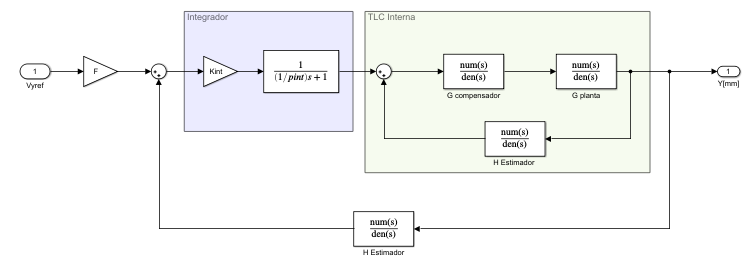
\includegraphics[scale=0.8]{Diagrama-en-bloques-comp.png}
	\caption{Diagrama del sistema completo.}
	\label{fig:diag-en-bloques-comp}
\end{figure}

\section{Lazo de realimentación interno}

\subsection{Análisis de estabilidad con masa de 30 kg}

\noindent Para realizar el análisis de estabilidad se parte de las transferencias de la planta $G_{p}(s)$ para una masa de 30 kg (\ref{eq_transferencia_planta_30kg}), de la del controlador de corriente $G_{iL}(s)$ (\ref{eq_TLC-cc}) y de la del lazo de realimentación $H_{estim}(s)$ (\ref{eq_TLC_deriv_7}). A partir de ellas se obtiene  la transferencia a lazo abierto total $GH_T(s)$ mostrada en la expresión \ref{eq_GT2}.

\begin{equation*} \label{eq_GT1}
	GH_T(s)=G_{p}(s)*G_{iL}(s)*H_{estim} 
\end{equation*}

\begin{equation} \label{eq_GT2}
		GH_T(s)=\frac{0.38}{(1-(\frac{s}{70})^2)(\frac{s}{12.17\ }+1)(1+\frac{s}{1\ Krad/s}){(1+\frac{s}{60\ Krad/s})}^2 }	
\end{equation}

\noindent A continuación se procede a analizar la respuesta en frecuencia de $GH_T$ y a diseñar un compensador adecuado. Luego, se verificará la estabilidad para una masa de $1\:kg$, que corresponde a la mínima con la que trabaja el sistema.


\noindent Con la transferencia de la ecuación  \ref{eq_GT2} se  grafica el diagrama de Bode y el diagrama de Nyquist. Estos se muestran en las figuras \ref{fig:Diag_Bode_lazo_abierto_30kg} y \ref{fig:Diag_Nyquist_lazo_abierto_30kg} respectivamente.

\begin{figure}[H]
	\centering
	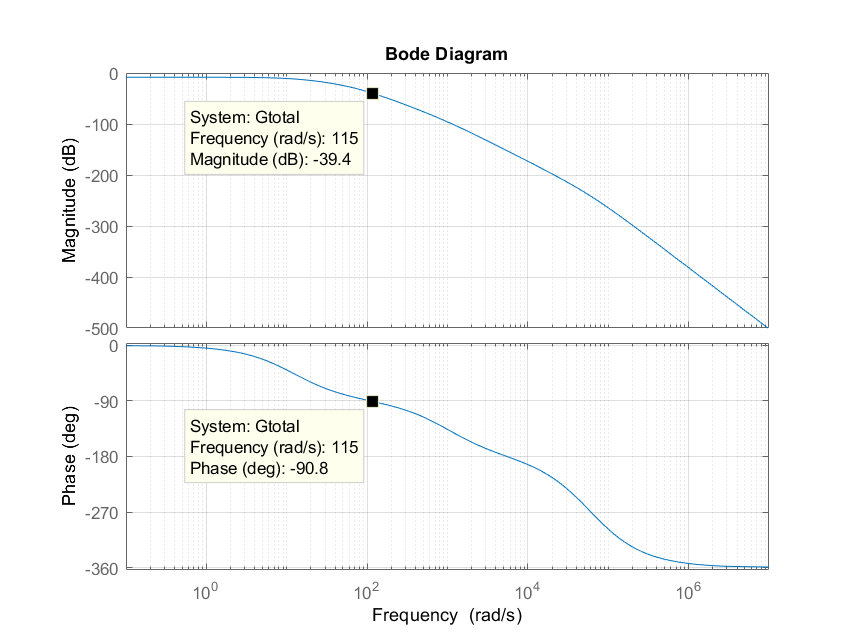
\includegraphics[scale=0.6]{bode_planta_30kg.png}
	\caption{Diagrama de Bode de lazo abierto $GH_T$ con $M=\:30 kg$.}
	\label{fig:Diag_Bode_lazo_abierto_30kg}
\end{figure}

\begin{figure}[H]
	\centering
	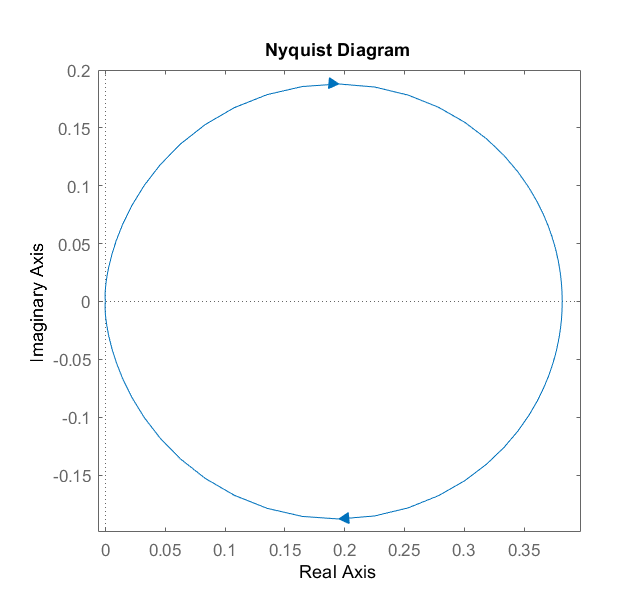
\includegraphics[scale=0.6]{nyquist_planta_30kg.png}
	\caption{Diagrama de Nyquist de $GH_T$ con $M=30\:kg$.}
	\label{fig:Diag_Nyquist_lazo_abierto_30kg}
\end{figure}

\noindent Para poder observar mejor la forma del Nyquist se hace un acercamiento en torno al origen como se muestra en la figura \ref{fig:Diag_Nyquist_lazo_abierto_zoom_30kg}.

\begin{figure}[H]
	\centering
	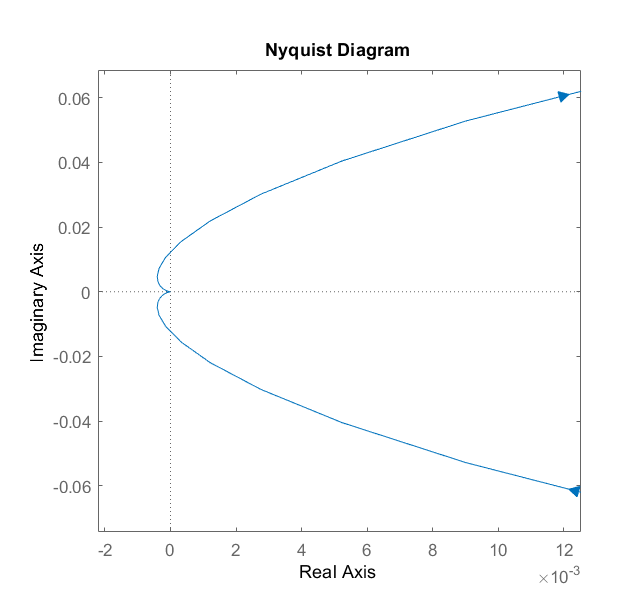
\includegraphics[scale=0.6]{nyquist_planta_zoom_30kg.png}
	\caption{Zoom del diagrama de Nyquist de $GH_T$ con $M=30\:kg$.}
	\label{fig:Diag_Nyquist_lazo_abierto_zoom_30kg}
\end{figure}

\noindent En la figura \ref{fig:rlocus_m30kg} se puede observar el lugar de raíces de $GH_{T}$ y en la \ref{fig:rlocus_m30kg_zoom} se muestra un acercamiento.

\begin{figure}[H]
	\centering
	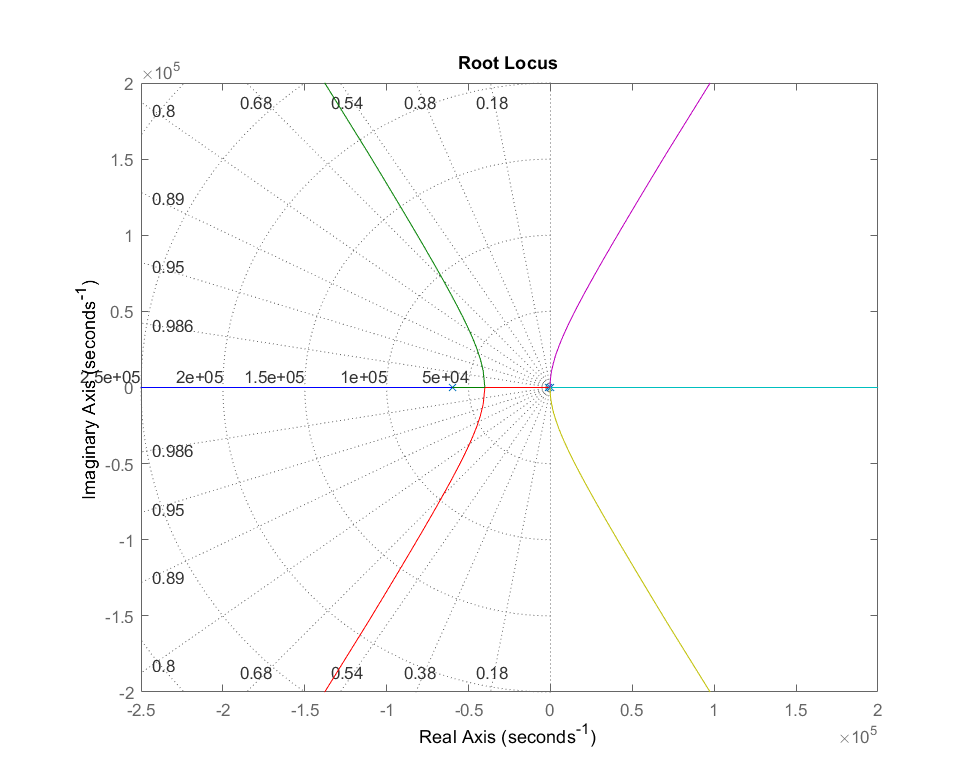
\includegraphics[scale=0.6]{rlocus_planta_30kg.png}
	\caption{Lugar de raíces de $GH_{T}$ con $M=30\:kg$.}
	\label{fig:rlocus_m30kg}
\end{figure}

\begin{figure}[H]
	\centering
	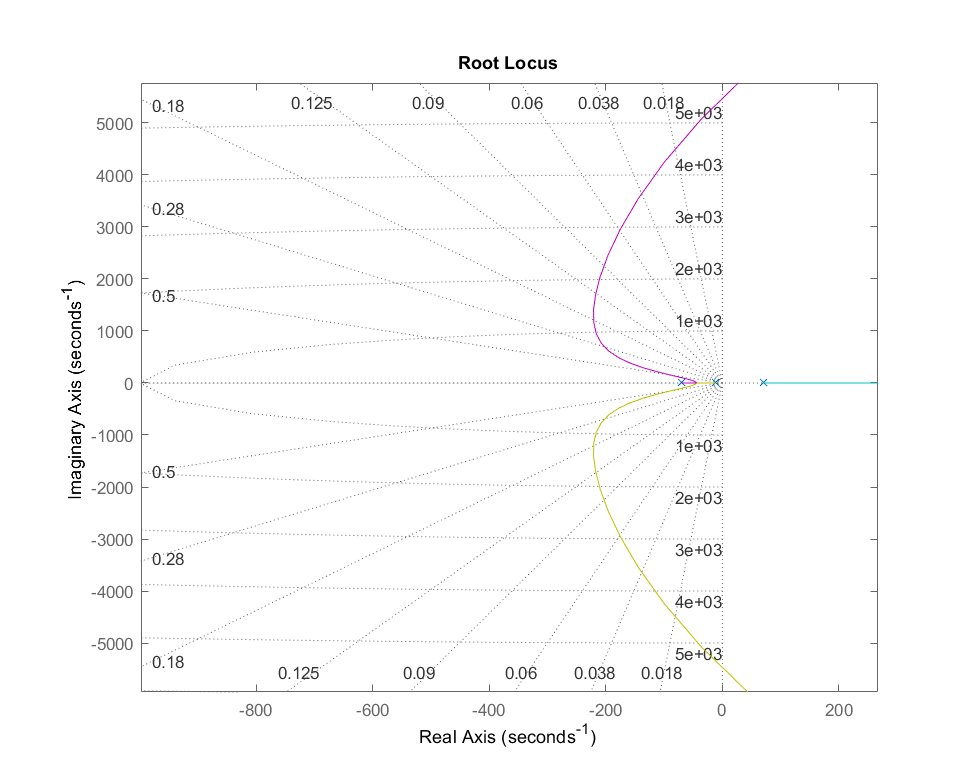
\includegraphics[scale=0.6]{rlocus_planta_30kg_zoom.png}
	\caption{Zoom del lugar de raíces de $GH_T$ con $M=30\:kg$.}
	\label{fig:rlocus_m30kg_zoom}
\end{figure}

\noindent Como se observa en la figura \ref{fig:rlocus_m30kg_zoom}, $GH_{T}$ tiene un polo en el semiplano derecho. Por lo tanto, a partir del Nyquist se puede determinar:

\noindent Zona 1: Z=N+P=0+1=1 $\mathrm{\to}$ Inestable 

\noindent Zona 2: Z=N+P=1+1=2 $\mathrm{\to}$ Inestable

\noindent Por lo tanto, no es posible que el sistema sea estable. Para lograrlo se realimentar\'{a} positivamente y se generar\'{a} una zona en el diagrama de Nyquist donde $N=-1$. Para ello es necesario aumentar la fase para que pueda superar el valor de 0$\mathrm{{}^\circ}$.  Para que esto se cumpla, el diagrama de Nyquist deber\'{i}a tener una forma como la  mostrada en la figura \ref{fig:nyquist-deseado-analog}.

\begin{figure}[H]
	\centering
	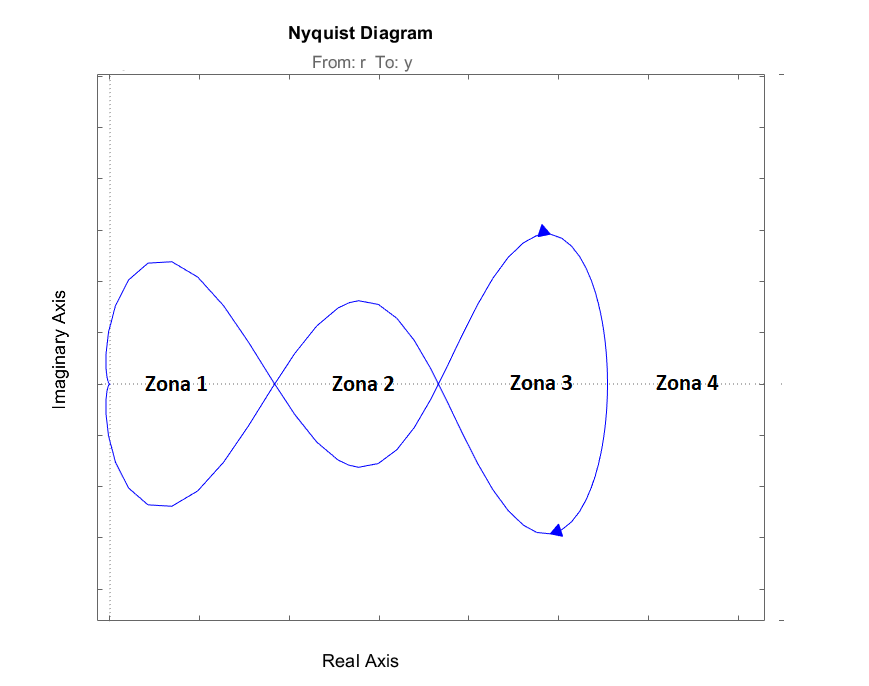
\includegraphics[scale=0.7]{Nyquist-deseado-analog.png}
	\caption{Forma del diagrama de Nyquist deseado.}
	\label{fig:nyquist-deseado-analog}
\end{figure}

\subsection{Diseño de la red de adelanto de fase}

\noindent Para poder lograr el aumento de fase mencionado se utiliza una red de adelanto de fase. Se debe tener en cuenta que el m\'{o}dulo de la transferencia de lazo abierto en el primer cruce de la fase por 0$\mathrm{{}^\circ}$ debe ser mayor a 0 dB y, en el segundo cruce, menor. De esta forma, al observar la figura \ref{fig:Diag_Bode_lazo_abierto_30kg} se decide adelantar la fase 100º en aproximadamente 200 rad/s. Esto se logra mediante el uso de dos redes de adelanto de fase de 65$\mathrm{{}^\circ}$ cada una.

\noindent Ecuaciones de dise\~{n}o:

\begin{equation*}
	\begin{aligned}
		W_0 &=200\ r/s\\
		{\varphi }_{max} &=65\textrm{º}\\
		\alpha &=\frac{1+sen{\varphi }_{max}}{1-sen{\varphi }_{max}}=20.346491\\
		W_c &=\frac{W_0}{\sqrt{\alpha }}=\ 44.3\ r/s\\
		W_p &=\sqrt{\alpha }*W_0=902.1\ r/s\\
	\end{aligned}
\end{equation*} 
\noindent Finalmente se llega a la transferencia del controlador:

\begin{equation}  
	G_c(s)=K*{[20.346*\frac{(s+44.3)}{(s+902.1)}]}^2
\end{equation} 

\noindent En la figura \ref{fig:bode-analog-compensado-para-k-1} se muestra el diagrama de bode de ${GH}_T*G_C$ con $K=1$. Se puede observar que la ganancia $K$ puede adoptar valores desde 15 dB hasta 35 dB. Al considerar que el sistema debe soportar una masa variable entre 1 kg y 30 kg, y que la ganancia de la transferencia de la planta para 1 kg es de 5.5 veces (14 dB) mayor que para 30 kg, se puede adoptar una ganancia del compensador que mantenga la estabilidad para estos dos casos. Es decir, la ganancia m\'{i}nima es de 15 dB y la m\'{a}xima es de 35 dB - 14 dB = 21 dB. Por lo tanto, se elige que el cruce por cero de la ganancia se encuentre ahora en 88 rad/s, lo que significa que $K=20dB\ \equiv \ 10\ veces$.


\begin{figure}[H]
	\centering
	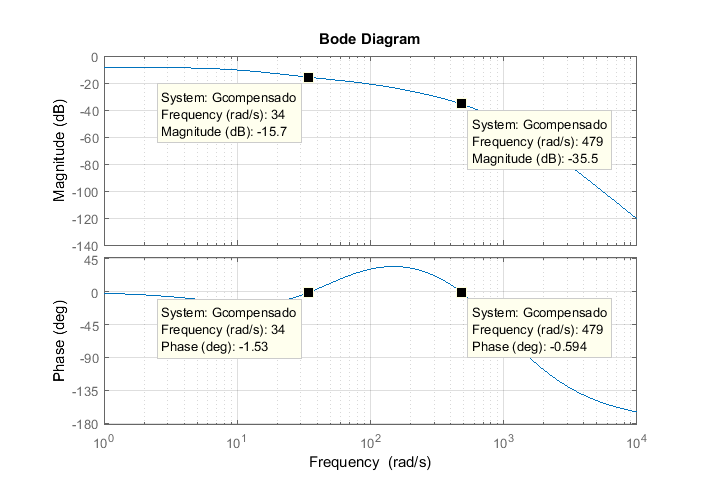
\includegraphics[scale=0.85]{Bode-k-1-M-30.png}
	\caption{Diagrama de Bode de $GH_T*G_C$ para K=1 y M=30 kg.}
	\label{fig:bode-analog-compensado-para-k-1}
\end{figure}

\noindent En la figura \ref{fig:bode-analog-compensado-para-k-10} se muestra el diagrama de Bode al considerar la ganancia del compensador. En ella se puede observar que se  cumple con el criterio de estabilidad, puesto que en el primer cruce por 0º, la magnitud es mayor a 0 dB y en el segundo cruce, menor. Adem\'{a}s, en la figura \ref{fig:nyquist-analog-para-k-10} se puede ver que la forma del diagrama de Nyquist es como la deseada.

\begin{figure}[H]
	\centering
	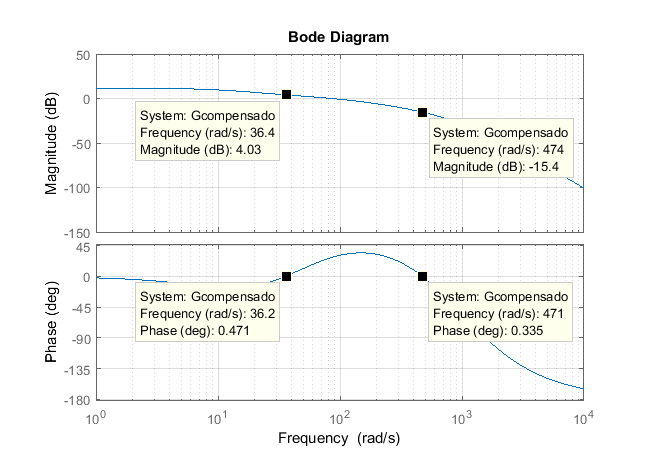
\includegraphics[scale=0.85]{Bode-k-10-M-30.png}
	\caption{Diagrama de Bode de $GH_{T}*G_C$ para K=10 y M=30 kg.}
	\label{fig:bode-analog-compensado-para-k-10}
\end{figure}

\begin{figure}[H]
	\centering
	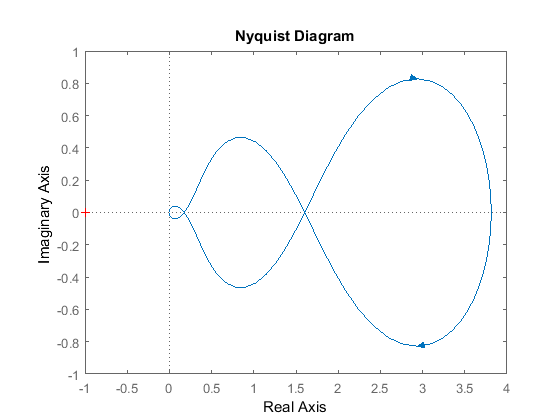
\includegraphics[scale=0.85]{Nyquist-k-10-M-30.png}
	\caption{Diagrama de Nyquist de $GH_T*G_C$ para K=10 y M=30 kg.}
	\label{fig:nyquist-analog-para-k-10}
\end{figure}

\noindent En la figura \ref{fig:rta-escalon-k-10-m-30} se puede observar la respuesta al escalón del sistema con masa de 30 Kg.

\begin{figure}[H]
	\centering
	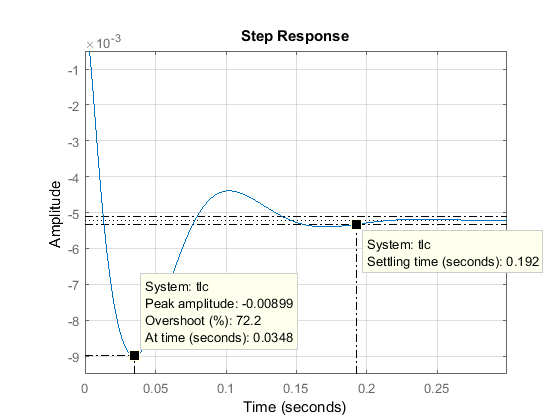
\includegraphics[scale=0.85]{Respuesta-al-escalon-K-10-M-30Kg.png}
	\caption{Respuesta al escalón para M=30 Kg.}
	\label{fig:rta-escalon-k-10-m-30}
\end{figure}

\subsection{Verificación de estabilidad con masa de 1 Kg}

\noindent Se verifica la estabilidad del sistema  para el caso en que la masa sea de 1 Kg con el compensador dise\~{n}ado para el caso de masa m\'{a}xima. Para ello, se analizan los diagramas de Bode y Nyquist mostrados en las figuras \ref{fig:bode-analog-para-M-1Kg} y \ref{fig:nyquist-analog-para-M-1Kg}. Adem\'{a}s, en la figura \ref{fig:respuesta-analog-al-escalon-para-M-1Kg} puede observarse la respuesta al escal\'{o}n. A partir de ellos, es posible verificar que el sistema resulta estable para todo el rango de masas en el que opera el sistema. 


\begin{figure}[H]
	\centering
	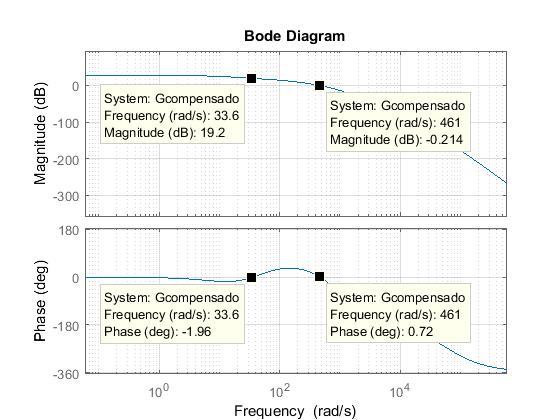
\includegraphics[scale=1]{bodecompensado1kg.png}
	\caption{Diagrama de Bode de $GH_T*G_C$ para M=1 Kg.}
	\label{fig:bode-analog-para-M-1Kg}
\end{figure}

\begin{figure}[H]
	\centering
	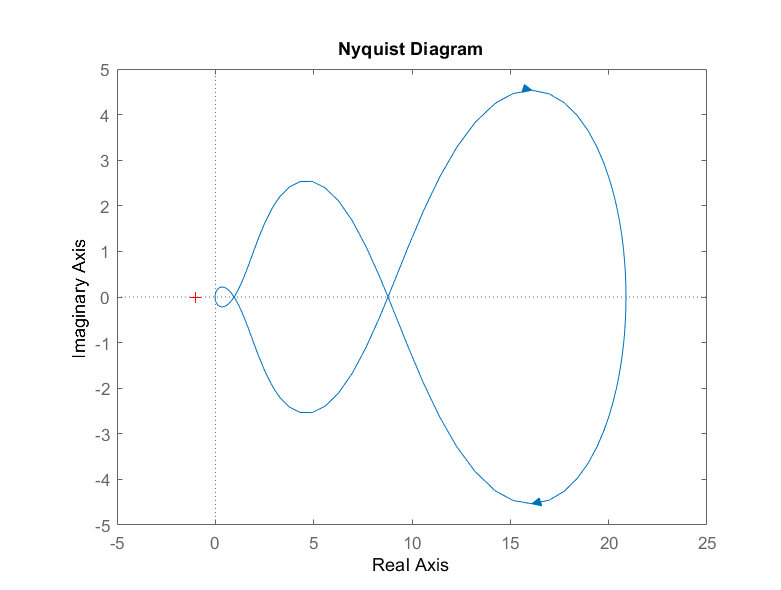
\includegraphics[scale=0.7]{nyquistcompensado1kg.png}
	\caption{Diagrama de Nyquist de $GH_T*GC$ para M=1 Kg.}
	\label{fig:nyquist-analog-para-M-1Kg}
\end{figure}

\begin{figure}[H]
	\centering
	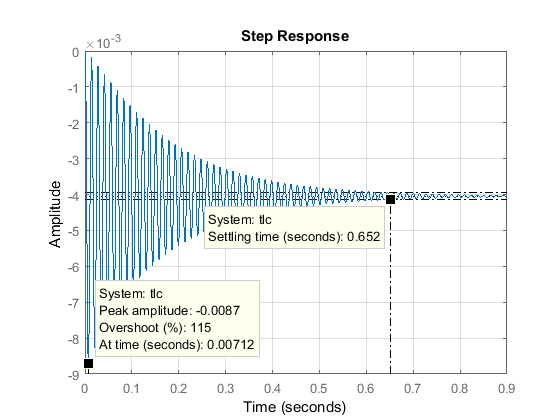
\includegraphics[scale=1]{rtaescaloncompensado1kg.png}
	\caption{Respuesta al escalón para M=1 Kg.}
	\label{fig:respuesta-analog-al-escalon-para-M-1Kg}
\end{figure}

\subsection{Implementación circuital de la red de adelanto de fase}

\begin{figure}[H]
	\centering
	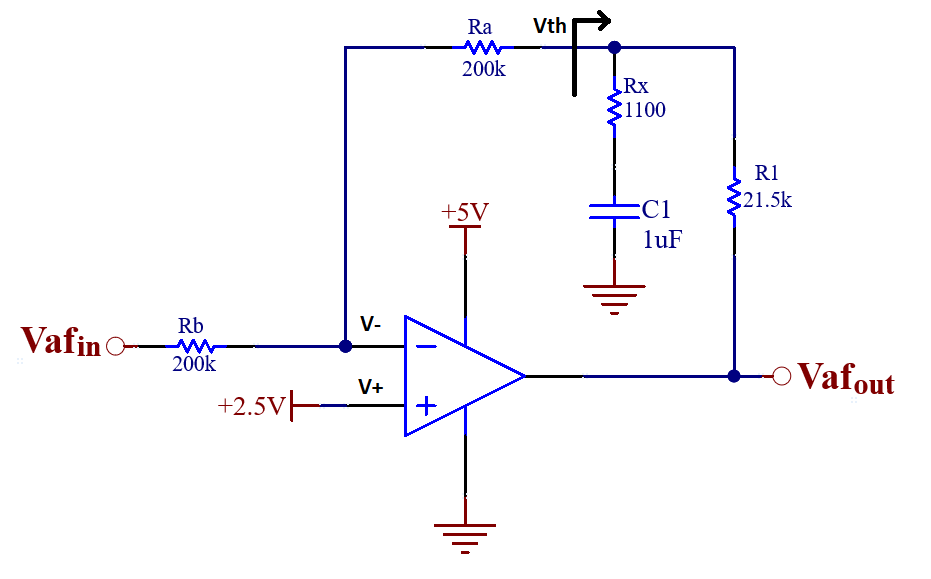
\includegraphics[scale=0.6]{Red-adelanto-fase.png}
	\caption{Diseño circuital de una red de adelanto de fase.}
	\label{fig:red-adelanto-fase}
\end{figure}


\noindent Para cada etapa del compensador por adelanto, se utiliza la topología mostrada en la figura \ref{fig:red-adelanto-fase}. Consiste en  un polo y cero con ganancia unitaria (si Ra = Rb). Luego se agrega la ganancia como una etapa separada.

\noindent La transferencia de lazo cerrado de esta etapa es:

\begin{equation} 
	\frac{V_{out}}{V_{in}}= - \frac{R_a}{R_b}*\frac{1+sC(R_x+R1)}{1+sCR_x}
\end{equation}

\noindent Por lo tanto, para tener un polo en $902.1\:Hz$ y un cero en $44.3\:Hz$, al elegir un capacitor $C = 1\:uF$, resulta en $R_x = 1100\:\Omega$ y $R1 = 21.5\:k\Omega$. Además, se elige $R_a = R_b = 200\:k\Omega$ para obtener una ganancia unitaria. Luego, la ganancia del compensador se obtiene con una etapa amplificadora.
Para ello, se utiliza el circuito mostrado en la figura \ref{fig:ganancia-compensador}. Para lograr una ganancia de K=10 se utiliza $R_{322} = 1\:k\Omega$ y $R_{323} = 10\:k\Omega$.


\begin{figure}[H]
	\centering
	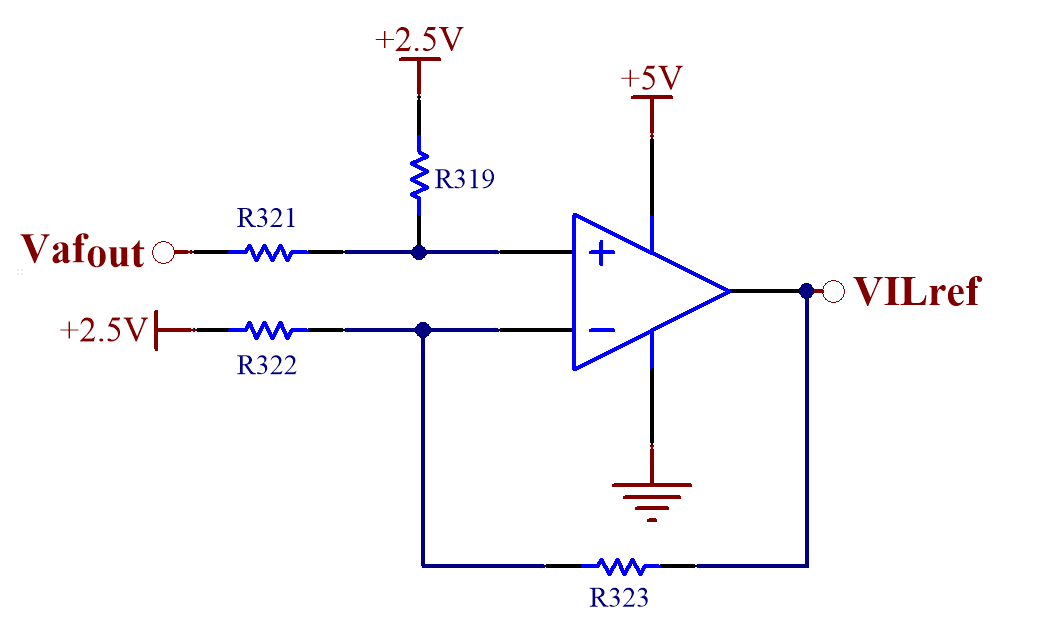
\includegraphics[scale=0.6]{Ganancia-compensador.png}
	\caption{Etapa de ganancia del compensador.}
	\label{fig:ganancia-compensador}
\end{figure}

\section{Lazo del realimentación externo}
\subsection{Diseño del integrador}

\noindent Se plantea un lazo de realimentaci\'{o}n externo como se muestra en la  figura \ref{fig:diag-en-bloques-comp}. En el lazo de realimentaci\'{o}n interno act\'{u}a el compensador por adelanto de fase dise\~{n}ado previamente y, en el externo, un controlador del tipo integral. De esta forma, se logra suavizar la respuesta al escal\'{o}n del sistema y eliminar el error en r\'{e}gimen permanente.


\noindent Para el an\'{a}lisis se considera como realimentaci\'{o}n: 

\[H_{estim}=\frac{V_{estim}}{Y[m]}= - \frac{259.6}{(1 + \frac{s}{1Kr/s})*(1+\frac{s}{60Kr/s})^2}\] 

\noindent La cadena de avance con masa de $30\:kg$ es:

\[G[m=30]=Tlc_{interna}(s)[m=30]*G_{integ}\] 

\noindent Se  plantea un compensador del tipo :

\[G_{integ}\ =\ k_{int}\ *\ \frac{1}{(1+(\frac{s}{p_{int}}))}\]

\noindent Debido a que un integrador con polo en el origen tiene una ganancia infinita en contínua, no sería adecuado implementarlo de esta manera en el circuito. Por lo tanto se ubica el polo en $0.1\:rad/s$ de forma tal que permita limitar dicha ganancia y ser de carácter integrativo para las frecuencias de la planta. Sin embargo, esta modificación provoca que la cancelación del error en régimen permanente no sea completa.
%, pero de todas maneras sea pequeña en comparación con la distancia de separación.

%Debido a que no usamos un integrador ideal, la respuesta al escalón presentará un cierto error.

Inicialmente se analiza la estabilidad del sistema con $K_{int} = 1$ por medio del lugar de raíces mostrado en la figura \ref{fig:lugar-de-raices-con-integrador-analog}.

\noindent Para este lazo de realimentación externo también debe utilizarse realimentación positiva, puesto que la TLC interna del sistema presenta una ganancia negativa.


\begin{figure}[H]
	\centering
	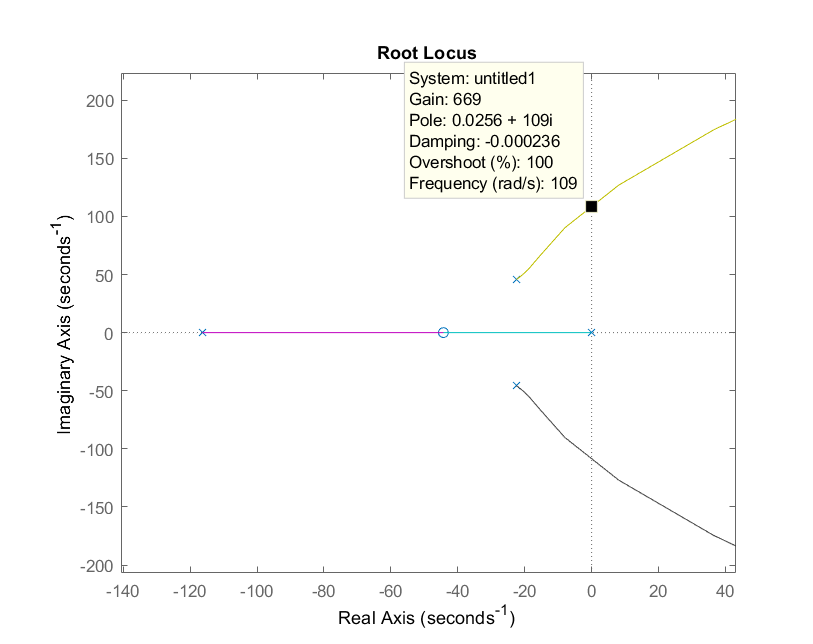
\includegraphics[scale=0.5]{rlocusconintegrador30kg.png}
	\caption{Lugar de raíces con el integrador.}
	\label{fig:lugar-de-raices-con-integrador-analog}
\end{figure}

\noindent En la figura \ref{fig:lugar-de-raices-con-integrador-analog} se puede observar que, para que se mantenga la estabilidad del sistema, la ganancia del integrador ($K_{int}$) debe ser menor a 669. Teniendo esto en cuenta, en la figura \ref{fig:respuesta-al-escalon-con-k-1-M-30-analog} se muestra la respuesta al escal\'{o}n del sistema compensado con el integrador para una ganancia de $K_{int\ }=1$.  Es posible observar que, si bien no presenta oscilaciones, el tiempo de establecimiento es de aproximadamente $16.6 \:s$ \colorbox{yellow}{Chequear, antes decía 3 seg pero creo que estaba mal}. Por lo tanto, se decide aumentar el valor de ganancia hasta obtener una relaci\'{o}n aceptable entre el tiempo de respuesta y el sobrepico.

\begin{figure}[H]
	\centering
	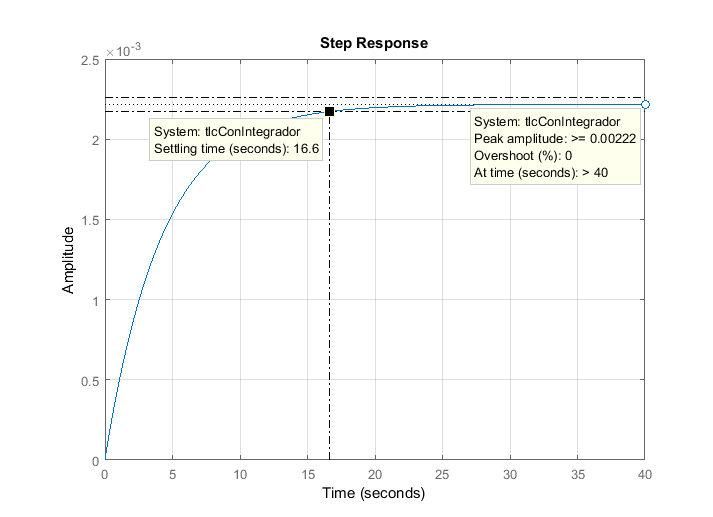
\includegraphics[scale=0.85]{stepresponseintegradorkint_1_m_30.png}
	\caption{Respuesta al escalón con integrador con $K_{int}$ =1 y M=30 Kg.}
	\label{fig:respuesta-al-escalon-con-k-1-M-30-analog}
\end{figure}

\noindent En la figura \ref{fig:respuesta-al-escalon-con-k-50-M-30}, se observa la respuesta al escal\'{o}n para una ganancia del integrador de $K_{int}=50$ que resulta en un tiempo de establecimiento de $0.6\:s$ y un overshoot de 0\%. Por lo tanto, se adopta este valor de ganancia para el dise\~{n}o del integrador.

\begin{figure}[H]
	\centering
	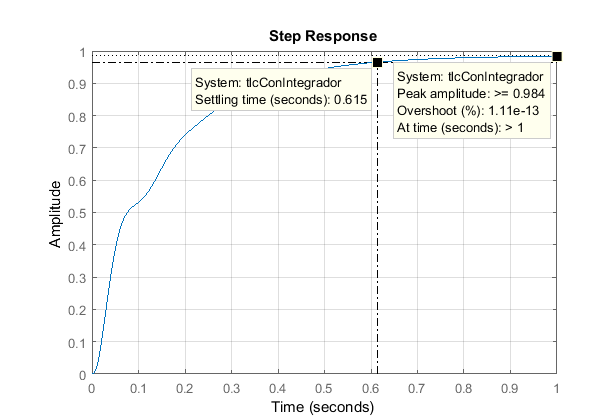
\includegraphics[scale=0.85]{stepresponseintegradorkint_50_m_30.png}
	\caption{Respuesta al escalón con integrador para $K_{int}$ =50 y M = 30 Kg.}
	\label{fig:respuesta-al-escalon-con-k-50-M-30}
\end{figure}

\noindent La respuesta al escal\'{o}n cuando la masa es de $1 \:kg$ se muestra en la figura \ref{fig:respuesta-al-escalon-con-k-50-M-1}. All\'{i} se puede observar que el tiempo de establecimiento es de $0.74\:s$ y que no presenta sobrepicos.

\begin{figure}[H]
	\centering
	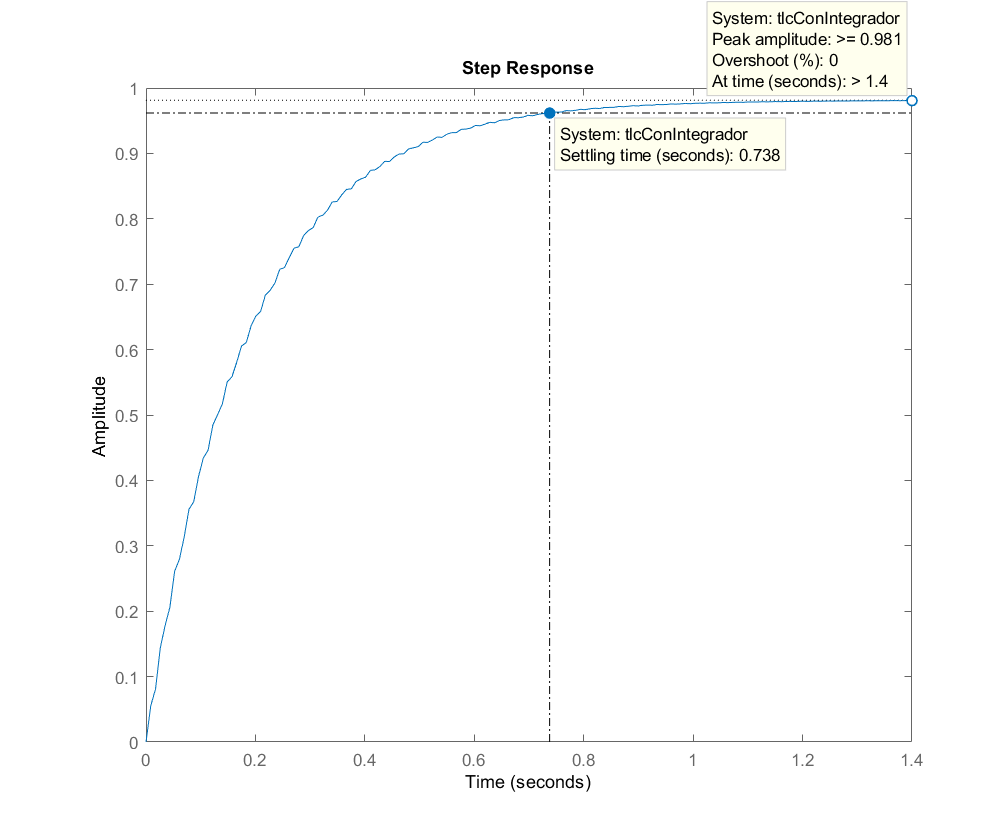
\includegraphics[scale=0.85]{stepresponseintegradorkint_50_m_1.png}
	\caption{Respuesta al escalón con integrador para $K_{int} =50$ y $M = 1 \:kg$.}
	\label{fig:respuesta-al-escalon-con-k-50-M-1}
\end{figure}



\subsection{Implementación circuital del integrador}

\noindent En la figura \ref{fig:circuito-integrador} se puede observar la topología y los valores utilizados en cada componente para el diseño del circuito integrador. 

\begin{figure}[H]
	\centering
	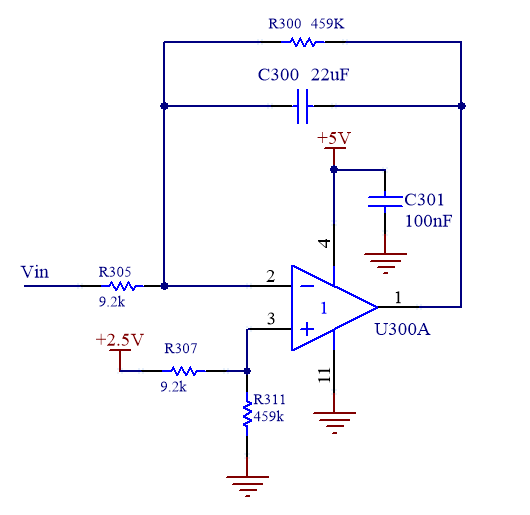
\includegraphics[scale=0.6]{Circuito-integrador.png}
	\caption{Implementación circuital del integrador.}
	\label{fig:circuito-integrador}
	\end{figure}
\section{Etapa de entrada}
\subsection{Cálculo de ganancia de entrada}

\noindent La ganancia de la TLC correspondiente a la ganancia total de los bloques con el integrador ya incorporado, resulta:

\begin{equation} 
	G_{TLC_{final}} \simeq \frac{1}{H_{estim}} = - \frac{1}{260}
\end{equation}

\begin{figure}[H]
	\centering
	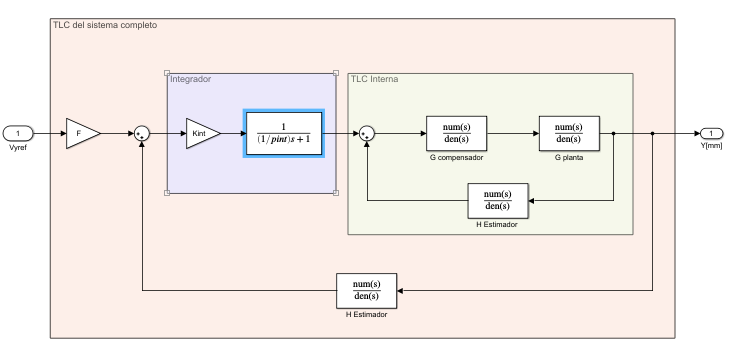
\includegraphics[scale=0.8]{Diagrama-en-bloques-compensador.png}
	\caption{Diagrama en bloques final.}
	\label{fig:diag-bloques-compensador}
\end{figure}

\noindent Por lo tanto, con $F=-1$ y los rangos de posición de $2\:mm$ a $5\:mm$ como mínimo y máximo respectivamente se llega a lo siguiente:

\begin{equation} 
	Y[m] = F * (-\frac{1}{260})*V_{in} =\frac{1}{260}*V_{in} 
\end{equation}

\noindent La realimentación tiene un set-point de $3.4\:V$ por lo tanto se le suma a $V_{in}$ el mismo valor.

\noindent Los valores finales son:


\begin{table}[H]
	\begin{center}
		\begin{tabular}{| c | c |}
			\hline
			Y[mm] & $V_{in}[V]$\\ \hline
			5 & 4.7\\ \hline
			4 & 4.44 \\ \hline
			3 & 4.18\\ \hline
			2 &	3.92 \\ \hline		
		\end{tabular}
		\caption{Tensión de referencia $[V_{in}]$ Vs separación deseada [Y].}
		\label{tension-ref-vs-separacion-deseada}
	\end{center}
\end{table}

\subsection{Implementación circuital}

\noindent Para poder modificar la distancia de separación se ingresa al sistema con una tensión variable, la cual corresponde a una posición de referencia. Para ello se utiliza el circuito mostrado en la figura \ref{fig:etapa-de-entrada}.

\begin{figure}[H]
	\centering
	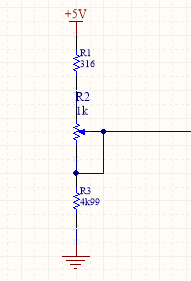
\includegraphics[scale=0.8]{Etapa-de-entrada.png}
	\caption{ Etapa de entrada.}
	\label{fig:etapa-de-entrada}
\end{figure}

 
 \noindent Se utiliza una resistencia variable de $1\:k\Omega$ y dos fijas. Para poder excursionar la tensión de referencia entre $3.92\:V$ y $4.7\:V$, los valores de las resistencias $R_1$ y $R_3$ deben ser de $4911\:\Omega$ y $313.5\:\Omega$ respectivamente. 
 
\noindent Por lo tanto, al adoptar un valor comercial para ellas, resulta en $R_1 = 316 \:\Omega$ y en $R_3 = 4990 \:\Omega$.
 
\noindent De esta forma, el valor de tensión máximo para la referencia de posición queda en $4.69\:V$ y el mínimo en $3.96\:V$.
 
